\documentclass[a4paper,10pt]{report}

\usepackage{ulsy}
\usepackage{amsmath,amssymb}
\usepackage{verbatim}
\usepackage{tikz}
\usepackage{ifthen}
\usepackage{alltt}
\usepackage{array}
\usepackage{wrapfig}
\usepackage{cancel}
\usepackage{graphicx}
\usepackage{algorithmic}
\usepackage{textcomp}
\usepackage{hyperref}
\usepackage{fixltx2e}
\usepackage{txfonts}
\usepackage{subfigure}
\usetikzlibrary{arrows,calc,positioning,shapes,matrix}

% Command for a standard citation needed superscript
\newcommand{\cn}[1][]{
    \textsuperscript{\textit{
        [citation needed\ifthenelse{\equal{#1}{}}{}{ - #1}]}}}

% Environment for code.
\newenvironment{code}{\small\verbatim}{\endverbatim}
% Advanced environment for code.  Requires the user to escape the characters \, {, and }.  However, allows LaTeX commands to be issued (like color) and preserves spaces.
\newenvironment{acode}{\small\begin{alltt}}{\end{alltt}}

% Environment for draft comments.
\newenvironment{draftcomment}{\vspace{0.5cm}\begin{itshape}\textbf{Draft comment: }}{\end{itshape}\vspace{0.5cm}}
\newcommand{\dc}[1]{\begin{draftcomment}#1\end{draftcomment}} % this makes comments less obvious... should we eliminate it?

% Shorthand for common escapes
\newcommand{\ttob}{{\tt\char'173}} % {
\newcommand{\ttcb}{{\tt\char'175}} % }
\newcommand{\ttbs}{{\tt\char'134}} % \
\newcommand{\ttsh}{{\tt\char'043}} % #
\newcommand{\ttca}{{\tt\char'136}} % ^

% Section reference macro
\newcommand{\refS}[1]{\hyperref[#1]{\S\ref{#1}}}

% Common text shortcuts (some of which are unnecessary but provide a nice point of abstraction)
\newcommand{\BSJ}{BSJ}
\newcommand{\JLS}{\textit{Java Language Specification}}
\newcommand{\opt}{\textsubscript{opt}}

% Vocabulary definition command
% TODO: create a glossary or index term or something?
\newcommand{\vocab}[1]{\textit{#1}}

% Change default second-level bullets
\renewcommand{\labelitemii}{$\vardiamondsuit$}

% Create an environment for grammar descriptions
% TODO: figure out how to make wrapped \item indent second and following lines (important for preamble syntax)
\newenvironment{grammar}{
    \begin{list}{}{
        \itshape
        \setlength{\partopsep}{\topsep}
        \setlength{\topsep}{0cm}
    }
}{
    \end{list}
}

\title{Backstage Java \textit{(draft)}}
\author{Zachary Palmer\\Joe Riley}

\begin{document}

\maketitle

\tableofcontents

\chapter*{Preface}
\label{secPreface}

\dc{TODO}

\chapter{Introduction}
\label{secIntro}

\dc{TODO}

\section{Terminology}
\label{secIntroTerms}

\dc{TODO: definitions of ``metaprogram'', ``object program'', ``stage'', etc.}

\section{Example Programs}
\label{secIntroExamples}

\dc{TODO}

\chapter{Grammar}
\label{secGrammar}

The BSJ language is a superset of the Java language; that is, any legal Java program is a legal BSJ program.  As a result, the lexical and syntactic structure of BSJ is very similar to that of Java.  Notation for the grammar presented within this document is given in \refS{secGrammarNotation}.  The few additions to lexical structure that exist are discussed in \refS{secGrammarLex}.  The syntax of BSJ is discussed throughout the remainder of this document and can be found in \refS{secMetaprog}, \refS{secDirectives}, and \refS{secCodelit}.

\section{Notation}
\label{secGrammarNotation}

As \BSJ{} is a supplement to the Java language, this document uses the same grammar format as the \JLS{}.  Each production for a rule is displayed on a single line, indented from the original rule declaration.  The suffix ``opt'' is used to refer to a part of a production which is optional.  For further information about this syntax, please consult \S{}2.4 of the \JLS.

For sake of convenience and illustration, this document will often include rules from the \JLS{} in modified and unmodified forms.  If a rule is included that has been changed from its presentation in the \JLS{}, its name is suffixed with the term ``\textit{modified}'' in parentheses.  If it has not been changed, its name is suffixed with the term ``\textit{unmodified}''.

\section{Lexical Structure}
\label{secGrammarLex}

\dc{TODO: discuss \#depends and other such keywords.  Note that many new symbols in BSJ (such as [:) are composed of existing Java lexical structure.}

\chapter{Metaprograms}
\label{secMetaprog}

A metaprogram is introduced in BSJ by the use of the \verb`[:` and \verb`:]` metaprogram declaration operators.  These operators may appear in any of the following locations:

\begin{itemize}
    \item At the top level of a compilation unit where a type declaration would normally appear.
    \item At the top level of a type declaration, such as immediately within a class or interface.
    \item Anywhere a statement may appear.
\end{itemize}

If the metaprogram declaration operators have no content (that is, they are separated only by whitespace), then the semantics of the metaprogram are the same as the semantics of a non-operation (\verb`;` in the Java syntax).  This fact is a consequence of the following rules but bears mentioning here for purposes of clarity and confirmation.

The formal syntactic effect of the above is illustrated below.  Some rules have been reproduced from the \JLS{} for convenience.

\begin{grammar}
    \item TypeDeclaration (modified):
    \begin{grammar}
        \item ClassDeclaration
        \item InterfaceDeclaration
        \item BsjMetaprogram
    \end{grammar}
\end{grammar}

\begin{grammar}
    \item ClassBodyDeclaration (modified):
    \begin{grammar}
        \item ClassMemberDeclaration
        \item InstanceInitializer
        \item StaticInitializer
        \item ConstructorDeclaration
        \item BsjMetaprogram
    \end{grammar}
\end{grammar}

\begin{grammar}
    \item InterfaceMemberDeclaration (modified):
    \begin{grammar}
        \item ConstantDeclaration
        \item AbstractMethodDeclaration
        \item ClassDeclaration
        \item InterfaceDeclaration
        \item BsjMetaprogram
        \item \verb`;`
    \end{grammar}
\end{grammar}

\begin{grammar}
    \item AnnotationTypeElementDeclaration (modified):
    \begin{grammar}
        \item AnnotationTypeElementDeclaration:
        \item AbstractMethodModifiers\opt{} Type Identifier \verb`(` \verb`)` DefaultValue\opt{} \verb`;`
        \item ConstantDeclaration
        \item ClassDeclaration
        \item InterfaceDeclaration
        \item EnumDeclaration
        \item AnnotationTypeDeclaration
        \item BsjMetaprogram
        \item \verb`;`
    \end{grammar}
\end{grammar}

\begin{grammar}
    \item BlockStatements (unmodified):
    \begin{grammar}
        \item BlockStatement
        \item BlockStatements BlockStatement
    \end{grammar}
\end{grammar}

\begin{grammar}
    \item BlockStatement (modified):
    \begin{grammar}
        \item LocalVariableDeclarationStatement
        \item ClassDeclaration
        \item BsjMetaprogram
        \item Statement
    \end{grammar}
\end{grammar}

\begin{grammar}
    \item BsjMetaprogram:
    \begin{grammar}
        \item \verb`[` \verb`:` Preamble\opt{} BlockStatements \verb`:` \verb`]`
    \end{grammar}
\end{grammar}

As demonstrated by the previous grammar description, a metaprogram consists of an optional preamble followed by a number of block statements.  The block statements are used as the body of the metaprogram to be executed.  The execution semantics of metaprograms are discussed in \refS{secCompExec}.

It should be noted that, like \verb`@interface`, the metaprogram start and end operators are comprised of two different tokens; that is, it is legal to write ``\verb`[ : :]`'' to indicate an empty metaprogram (using a space between the bracket and colon).  For clarity, however, this should not be done in practice.  This allows parsers with a rigid set of assumptions about the Java language to be more easily adapted to parsing BSJ.

\section{Preamble}
\label{secMetaprogPreamble}

The metaprogram preamble allows the metaprogrammer to define attributes of the metaprogram (the metaprogram metadata).  These attributes control the execution semantics and the execution order of the metaprograms in a compilation unit.  A preamble consists of a number of preamble statements; preamble statements always begin with a preamble statement keyword.  To avoid collision with the existing Java namespace, preamble statements are always prefixed with the hash sign (\verb`#`) which does not appear anywhere in the syntax of the Java language itself.

\begin{grammar}
    \item Preamble:
    \begin{grammar}
        \item
            MetaprogramImportDeclarationList\opt{}
            MetaprogramModeDeclaration\opt{}
            MetaprogramTargetDeclaration\opt{}
            MetaprogramDependencyDeclaration\opt{}
    \end{grammar}
\end{grammar}

\subsection{Metaprogram Imports}
\label{secMetaprogPreambleImports}

Metaprogram imports take on the same form as normal imports except with the \verb`#import` keyword in place of the \verb`import` keyword.  The body of the metaprogram reacts to the metaprogram import in the same way that the body of an object program reacts to a normal import.

\begin{grammar}
    \item MetaprogramImportDeclarationList:
    \begin{grammar}
        \item MetaprogramImportDeclaration
        \item MetaprogramImportDeclarationList MetaprogramImportDeclaration
    \end{grammar}
\end{grammar}

\begin{grammar}
    \item MetaprogramImportDeclaration:
    \begin{grammar}
        \item \verb`#import` MetaprogramImportBody \verb`;`
    \end{grammar}
\end{grammar}

\begin{grammar}
    \item MetaprogramImportBody:
    \begin{grammar}
        \item TypeName
        \item PackageOrTypeName \verb`.` \verb`*`
        \item \verb`static` TypeName \verb`.` Identifier
        \item \verb`static` TypeName \verb`.` \verb`*`
    \end{grammar}
\end{grammar}

As a form of syntactic sugar, metaprogram imports may also appear in the import declarations section of a compilation unit.  Placing a metaprogram import statement in the compilation unit's import declarations is eqvuialent to placing that same metaprogram import statement in the preamble of every metaprogram contained in that source unit.  Such a metaprogram import is termed a ``global metaprogram import.''  For instance, the compilation unit

\begin{code}
#import com.example.*;
public class Example {
    [:
        foo();
    :]
}
[:
    bar();
:]
\end{code}

is equivalent to the compilation unit

\begin{code}
public class Example {
    [:
        #import com.example.*;
        foo();
    :]
}
[:
    #import com.example.*;
    bar();
:]
\end{code}

If a metaprogram introduces another metaprogram to the compilation unit, the latter metaprogram's global imports are determined after the prior metaprogram's execution terminates.  If the prior metaprogram adds or removes global metaprogram imports to or from the compilation unit, those modifications will affect the latter metaprogram; this is true whether the prior metaprogram modified the global metaprogram imports first or added the latter metaprogram first.

In addition to the imports already listed, the following imports are assumed for every metaprogram:

{\ttfamily
\begin{itemize}
    \item edu.jhu.cs.bsj.compiler.ast.*
    \item edu.jhu.cs.bsj.compiler.ast.node.*
    \item edu.jhu.cs.bsj.compiler.ast.node.meta.*
    \item edu.jhu.cs.bsj.compiler.metaprogram.*
\end{itemize}
}

\subsection{Mode Declarations}
\label{secMetaprogPreambleMode}

The operational mode of a metaprogram affects the nodes it can access and modify.  By default, metaprograms operate in \texttt{normal} mode, giving them the ability to perform a restricted set of modifications to their peers and the ability to read any node in the AST.  This is done to limit the scope of impact that metaprograms have and prevent counterintuitive side effects.

In some cases, however, metaprograms require the freedom to arbitrarily mutate some nodes or to perform insertions outside of their normal scope.  In this case, a mode declaration can be provided which alters the metaprogram's mode of operation.  A full discussion of metaprogram modes is found in \refS{secMetaprogModes}.

\begin{grammar}
    \item MetaprogramModeDeclaration:
    \begin{grammar}
        \item \verb`#mode` MetaprogramModeList \verb`;`
    \end{grammar}
\end{grammar}

\begin{grammar}
    \item MetaprogramModeList
    \begin{grammar}
        \item MetaprogramMode
        \item MetaprogramModeList \verb`,` MetaprogramMode
    \end{grammar}
\end{grammar}

\begin{grammar}
    \item MetaprogramMode:
    \begin{grammar}
        \item MetaprogramLocalMode
        \item MetaprogramPackageMode
    \end{grammar}
\end{grammar}

\begin{grammar}
    \item MetaprogramLocalMode:
    \begin{grammar}
        \item \verb`readOnly`
        \item \verb`insert`
        \item \verb`mutate`
        \item \verb`fullMutate`
    \end{grammar}
\end{grammar}

\begin{grammar}
    \item MetaprogramPackageMode:
    \begin{grammar}
        \item \verb`packageRead`
        \item \verb`packageInsert`
    \end{grammar}
\end{grammar}


It should be noted that none of the metaprogram modes are keywords in BSJ; they may be used as variable names, method names, and so on just as in Java.  Mode names are always lexically compatible with identifiers and may be tokenized as such, but a parser is obligated to produce an AST which contains only legal modes.

\subsection{Dependency Declarations}
\label{secMetaprogPreambleDeps}

Metaprogram dependency declarations control the order in which metaprograms run.  Each metaprogram has a \vocab{target} which groups it with other metaprograms for purposes of execution.  Metaprograms can also depend upon targets; these dependencies form the basis of the execution order.  See \refS{secMetaprogDeps} for a complete explanation of the semantic meaning of these declarations.

\begin{grammar}
    \item MetaprogramDependencyDeclaration:
    \begin{grammar}
        \item \verb`#depends` MetaprogramTargetNameList \verb`,`\opt{} \verb`;`
    \end{grammar}
\end{grammar}

\begin{grammar}
    \item MetaprogramTargetNameList:
    \begin{grammar}
        \item MetaprogramTargetName
        \item MetaprogramTargetNameList \verb`,` MetaprogramTargetName
    \end{grammar}
\end{grammar}

\begin{grammar}
    \item MetaprogramTargetDeclaration:
    \begin{grammar}
        \item \verb`#target` MetaprogramIdentifierList \verb`,`\opt{} \verb`;`
    \end{grammar}
\end{grammar}

\begin{grammar}
    \item MetaprogramIdentifierList:
    \begin{grammar}
        \item Identifier
        \item MetaprogramIdentifierList \verb`,` Identifier
    \end{grammar}
\end{grammar}

The syntax and semantics of \textit{MetaprogramTargetName} are discussed in \refS{secMetaprogNames}.

\section{Dependencies}
\label{secMetaprogDeps}

Due to the fact that they are operating on the same data structure, the order of metaprogram execution may have significant impact on the semantics of the resulting object program.  As a result, metaprograms are capable of specifying their dependencies upon other metaprograms.  A BSJ compiler provides support for ensuring that metaprograms are run in the correct order, detecting cycles in the metaprogram dependency graph, and detecting some occasions in which the expressed dependencies are incorrect (typically in the form of detecting a dependency which was not listed).

Metaprograms have (among their various metadata) unique identities, targets, and dependencies.  The unique identities of metaprograms are implementation-specific and not user-specified.  A target is a set of metaprograms; a metaprogram target declaration indicates that the metaprogram is part of the specified target.  A dependency indicates that the metaprogram must be executed after all metaprograms in the target on which it depends.  If a metaprogram does not declare a target, it is part of its own unique target on which no metaprogram can depend.

For example, consider the following sequence of metaprograms:

\begin{code}
    [: #target X; :]              // metaprogram A
    [: #target X; :]              // metaprogram B
    [: #target X, Y; :]           // metaprogram C
    [: #target Z; #depends X; :]  // metaprogram D
    [: #target Z; #depends Y; :]  // metaprogram E
    [: #depends Z; :]             // metaprogram F
    [: :]                         // metaprogram G
\end{code}

The names given to each of these metaprograms in the comments are arbitrary and solely for the purposes of the following discussion; the BSJ compiler is under no obligation to use those names or generate anything similar to them.  These metaprograms form the directed dependency graph shown in Figure \ref{figureDepGraphExample}.

\begin{figure}
    \begin{center}
        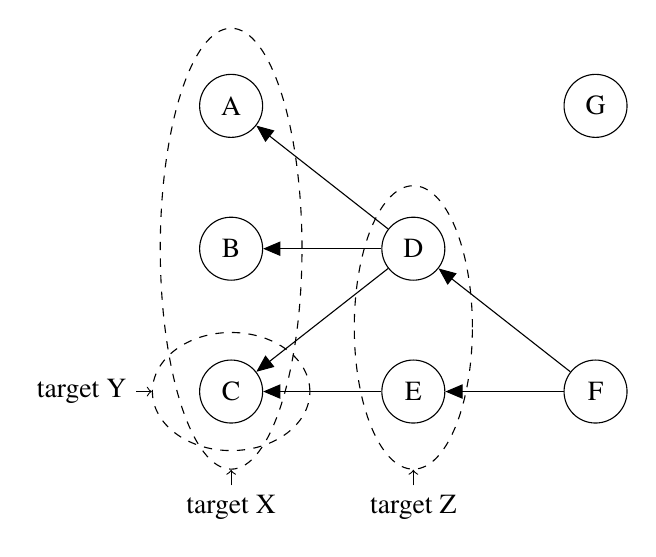
\begin{tikzpicture}[node distance=1cm and 1.5cm]
            \tikzstyle{node} = [draw,circle,minimum width=8mm]
            \tikzstyle{edge} = [-triangle 45]
            
            \node[node] (A) {A};
            \node[node] (B) [below=of A] {B};
            \node[node] (C) [below=of B] {C};
            \node[node] (D) [right=of B] {D};
            \node[node] (E) [right=of C] {E};
            \node[node] (F) [right=of E] {F};
            \node[circle,minimum width=8mm] (spacer) [right=of A] {};
            \node[node] (G) [right=of spacer] {G};
            
            \draw[edge] (D) -- (A);
            \draw[edge] (D) -- (B);
            \draw[edge] (D) -- (C);
            \draw[edge] (E) -- (C);
            \draw[edge] (F) -- (D);
            \draw[edge] (F) -- (E);
            
            \begin{scope}[node distance=2mm and 2mm]
                \node[draw,ellipse,minimum width=18mm,minimum height=56mm,dashed] (X) at (B) {};
                \node[] (X-label) [below=of X] {target X};
                \draw[->] (X-label) -- (X);
                \node[draw,ellipse,minimum width=20mm,minimum height=15mm,dashed] (Y) at (C) {};
                \node[] (Y-label) [left=of Y] {target Y};
                \draw[->] (Y-label) -- (Y);
                \node[draw,ellipse,minimum width=15mm,minimum height=36mm,dashed] (Z) at ($(D) - (0,1)$) {};
                \node[] (Z-label) [below=of Z] {target Z};
                \draw[->] (Z-label) -- (Z);
            \end{scope}
        \end{tikzpicture}
    \end{center}
    \caption{Dependency Graph Example}
    \label{figureDepGraphExample}
\end{figure}

For example, the graph shows a direct path from metaprogram D to metaprogram A; this indicates that metaprogram A must execute before metaprogram D.  More indirectly, metaprogram F is required to execute before metaprogram C because a path exists from F to C.  Note that no path containing metaprogram G contains any other metaprograms; thus, metaprogram G may execute in any order with respect to the other metaprograms.

If the preambles of metaprograms in the program being compiled construct a dependency graph which contains a cycle, a compile-time error occurs.

\subsection{Conflicts}
\label{secMetaprogDepsConflicts}

The purpose of metaprogram dependencies is to allow metaprograms to be executed in an explicit order when necessary as execution order can clearly affect the semantics of a metaprogram.  If, for instance, metaprogram A adds a field to a class declaration and metaprogram B iterates over the fields of that class declaration to generate an implementation of \verb`toString()`, whether metaprogram A executes before or after metaprogram B has an impact on the \verb`toString()` method that is generated.

BSJ provides the dependency system not only to permit control over metaprogram execution order but also to require that metaprogram execution order is controlled.  When two metaprograms may potentially operate in a conflicting manner, their execution order must be explicitly specified or a compile-time error occurs.  In this way, the order in which the BSJ compiler chooses to execute the metaprograms does not affect the object program which is generated; either the object program is generated (in which case only one object program could be generated for the given dependency graph and metaprogram runtime input) or no object program is generated (due to the compile-time error).  The latter case is said to represent a \vocab{conflict} of at least two metaprograms.

In order to define conflicts precisely, we require definitions of two terms: \vocab{attributes} and \vocab{cooperation}.  Each node in an AST has a set of attributes.  For most nodes, there is a one-to-one correspondence between attributes and properties.  (For a complete discussion of attributes, see \refS{setMetaprogDepsAtts}.)  Each time an attribute on an AST is accessed, it is accessed in either a \textit{read} or \textit{write} fashion.  This type of access is recorded along with the attribute, the node, and the identity of the metaprogram.

Two metaprograms are said to cooperate if there is an explicit dependency order between them.  More formally, two metaprograms cooperate if and only if there exists some path on the metaprogram dependency graph which contains both metaprograms.  Cooperation of metaprograms ensures that they can be executed in only one order, preventing any actions they take from conflicting with each other.

A conflict is then defined as any pair of accesses for which the following are all true:
\begin{itemize}
    \item Both accesses refer to the same attribute and the same node.
    \item The metaprograms of each access do not cooperate with each other.
    \item At least one of the accesses is a \textit{write}.
\end{itemize}

\subsection{Attributes}
\label{secMetaprogDepsAtts}

Most nodes have exactly one attribute per property.  For instance, a \verb`BinaryExpressionNode` has three attributes: one for the left operand, one for the right operand, and one for the binary operator applied to the operands.  The only exceptions to this rule are the descendents of the \verb`ListNode` class and the \verb`PackageNode` class.

\subsubsection{ListNode}
\label{secMetaprogDepsAttsList}

The number of attributes contained in a \verb`ListNode` is proportional to the number of elements in the list.  Each element in a \verb`ListNode` is associated with three attributes: \textit{Before}, \textit{After}, and \textit{Present}.  The \textit{Before} attribute for a given element is the same as the \textit{After} attribute for the preceding element.  In addition, each list contains an extra \textit{Size} attribute for the size of the list itself.

For example, a single element list has four attributes: a \textit{Before}, a \textit{Present}, an \textit{After}, and a \textit{Size}.  A two element list has six: a \textit{Before}, a \textit{Present} for the first element, an \textit{After} for the first element (which serves as the \textit{Before} of the second), a \textit{Present} for the second element, an \textit{After} for the second element , and a \textit{Size}.  An empty list has two attributes: a single \textit{Before} (which might have events logged on it if, for instance, an element were added to and then removed from the list) and a \textit{Size}.

Operations on a list node concern two varieties of elements: order-dependent and order-independent.  Whether an element is order-dependent or not depends both on the type of node and the type of the list.  The following cases are order-dependent:

\begin{itemize}
    \item Any element contained in a list of the following types:
    \begin{itemize}
        \item \verb`AnnotationElementListNode`
        \item \verb`AnnotationValueListNode`
        \item \verb`BlockStatementListNode`
        \item \verb`CaseListNode`
        \item \verb`CatchListNode`
        \item \verb`DeclaredTypeListNode`
        \item \verb`EnumConstantDeclarationListNode`
        \item \verb`ExpressionListNode`
        \item \verb`ReferenceTypeListNode`
        \item \verb`StatementExpressionListNode`
        \item \verb`TypeArgumentListNode`
        \item \verb`TypeParameterListNode`
        \item \verb`VariableDeclaratorListNode`
        \item \verb`VariableInitializerListNode`
        \item \verb`VariableListNode`
    \end{itemize}
    \item Any element which is an \verb`InitializerDeclarationNode`.
\end{itemize}

Whenever an element is added to or removed from a list, a write operation is logged against that element's \textit{Present} and \textit{Size} attributes.  Additionally, if the element is order-dependent, a write operation is logged against the element's \textit{Before} and \textit{After} attributes.  It is critical that these operations are applied even if the removal of the element from the list would remove the attribute from the list as well.

Whenever an element in a list is accessed, a read operation is logged only against the \textit{Present} attribute.  The \textit{Before} and \textit{After} attributes are unaffected.  Whenever the size of a list is accessed directly, a read operation is logged against the \textit{Size} attribute.

For example, consider Figure \ref{figureAttributeExample}, which represents the following sequence of accesses to an initially empty list:

\begin{enumerate}
    \item Add child \textbf{A} to the list.
    \item Add child \textbf{B} to the end of the list.
    \item Remove child \textbf{A} from the list.
    \item Add child \textbf{A} to the end of the list.
\end{enumerate}

\begin{figure}
    \begin{center}
        \tikzstyle{between} = [draw,circle,minimum width=2mm,fill=black,inner sep=0cm]
        \tikzstyle{element} = [draw,rectangle,minimum width=8mm,minimum height=8mm]
        \tikzstyle{edge} = []
        \tikzstyle{uid} = []
        \subfigure[After step 1]{
            \begin{tikzpicture}[node distance=5mm and 5mm]
                \matrix[ampersand replacement=\&,row sep=2mm,column sep=5mm] (list) {
                    \node[uid] {1}; \&
                    \node[uid] {2}; \&
                    \node[uid] {3}; \\
                    \node[between] (a0b) {};
                    \&
                    \node[element] (a0) {A};
                    \&
                    \node[between] (a1b) {};
                    \\
                };
                
                \draw[edge] (a0b) -- (a0);
                \draw[edge] (a0) -- (a1b);
                
                \node [below=of list,anchor=south] {\small Writes: 1, 2, 3.};
            \end{tikzpicture}
        }
        \hspace{5mm}
        \subfigure[After step 2]{
            \begin{tikzpicture}[node distance=5mm and 5mm]
                \matrix[ampersand replacement=\&,row sep=2mm,column sep=5mm] (list) {
                    \node[uid] {1}; \&
                    \node[uid] {2}; \&
                    \node[uid] {4}; \&
                    \node[uid] {5}; \&
                    \node[uid] {3}; \\
                    \node[between] (a0b) {};
                    \&
                    \node[element] (a0) {A};
                    \&
                    \node[between] (a1b) {};
                    \&
                    \node[element] (a1) {B};
                    \&
                    \node[between] (a2b) {};
                    \\
                };
                
                \draw[edge] (a0b) -- (a0);
                \draw[edge] (a0) -- (a1b);
                \draw[edge] (a1b) -- (a1);
                \draw[edge] (a1) -- (a2b);
                
                \node [below=of list,anchor=south] {\small Writes: 4, 5, 3.};
            \end{tikzpicture}
        }
        \\
        \subfigure[After step 3]{
            \begin{tikzpicture}[node distance=5mm and 5mm]
                \matrix[ampersand replacement=\&,row sep=2mm,column sep=5mm] (list) {
                    \node[uid] {4}; \&
                    \node[uid] {5}; \&
                    \node[uid] {3}; \\
                    \node[between] (a1b) {};
                    \&
                    \node[element] (a1) {B};
                    \&
                    \node[between] (a2b) {};
                    \\
                };
                
                \draw[edge] (a1b) -- (a1);
                \draw[edge] (a1) -- (a2b);
                
                \node [below=of list,anchor=south] {\small Writes: 1, 2, 4.};
            \end{tikzpicture}
        }
        \hspace{5mm}
        \subfigure[After step 4]{
            \begin{tikzpicture}[node distance=5mm and 5mm]
                \matrix[ampersand replacement=\&,row sep=2mm,column sep=5mm] (list) {
                    \node[uid] {4}; \&
                    \node[uid] {5}; \&
                    \node[uid] {6}; \&
                    \node[uid] {7}; \&
                    \node[uid] {3}; \\
                    \node[between] (a1b) {};
                    \&
                    \node[element] (a1) {B};
                    \&
                    \node[between] (a2b) {};
                    \&
                    \node[element] (a2) {A};
                    \&
                    \node[between] (a3b) {};
                    \\
                };
                
                \draw[edge] (a1b) -- (a1);
                \draw[edge] (a1) -- (a2b);
                \draw[edge] (a2b) -- (a2);
                \draw[edge] (a2) -- (a3b);
                
                \node [below=of list,anchor=south] {\small Writes: 3, 6, 7.};
            \end{tikzpicture}
        }
    \end{center}
    \caption{Attribute Access Example.  Boxes represent list elements and the corresponding presence attributes; dots represent before or after attributes.  UIDs for the attributes are indicated above the attribute symbol.  Text below the diagrams indicates which attributes have been written during that step.}
    \label{figureAttributeExample}
\end{figure}

Observe that, although the child node A was added back to the list in step 4, the attributes associated with it are new.  If the fourth step were performed by a different metaprogram, a conflict would occur because both metaprograms performed write operations on the list node's attribute with UID 3.

\subsubsection{PackageNode}
\label{secMetaprogDepsAttsPackage}

Nodes of type \verb`PackageNode` also have numerous attributes.  Package nodes only permit the addition of children; children cannot be removed from them.  Children are of one of two types: compilation units or immediate subpackages.  Children are keyed by their names.  Therefore, one attribute exists for each possible name.  Each addition of a child causes a write operation to the attribute corresponding to the child's name; each access (through iteration or through direct request) causes a read operation to the same attribute.

\section{Target Names}
\label{secMetaprogNames}

\S{}6.5 of the \JLS{} specifies the procedure used to determine the meaning of a name in the Java language.  Initially, names are placed in one of six categories.  The BSJ language introduces a seventh category of name: \textit{MetaprogramTargetName}.  The syntax for a metaprogram target name is similar to that of other names in the Java language:

\begin{grammar}
    \item MetaprogramTargetName:
    \begin{grammar}
        \item Identifier
        \item TypeName \verb`.` Identifier
    \end{grammar}
\end{grammar}

Once names are initially categorized, the rules in \S{}6.5.1 of the \JLS{} indicate how names are classified according to context.  Metaprogram targets are discussed in two locations in the BSJ language: in metaprogram target declarations and in metaprogram dependency declarations.  When a target is declared, it may not be qualified; as a result, it is impossible for a metaprogram target name to appear in a metaprogram target declaration.  When a metaprogram dependency is declared, the provided name is always unambiguously a \textit{MetaprogramTargetName}.  Thus, the following amendment to \S{}6.5.1 applies:

\begin{quote}
    A name is syntactically qualified as a \textit{MetaprogramTargetName} in these contexts:
    \begin{itemize}
        \item In a metaprogram dependency declaration (\refS{secMetaprogPreambleDeps}).
    \end{itemize}
    
    A name is syntactically qualified as a \textit{TypeName} in these contexts:
    \begin{itemize}
        \item To the left of a \verb`.` in a \textit{MetaprogramTargetName}.
    \end{itemize}
\end{quote}

Metaprogram target names are declared by the use of the \textit{MetaprogramTargetDeclaration} (\refS{secMetaprogPreambleDeps}) and explicitly indicate only the trailing identifier.  If the metaprogram target has a qualified name, that name is inferred based on the location of the metaprogram (\refS{secMetaprogNamesQual}).  When a \textit{MetaprogramDependencyDeclaration} (\refS{secMetaprogPreambleDeps}) is issued, it may either use that qualified name or a simple name, the latter of which is interpreted according to the rules in \refS{secMetaprogNamesDepnames}.

As indicated in \refS{secMetaprogDeps}, it is legal for multiple metaprograms to share the same target.  It is also legal for a metaprogram to participate in multiple targets.  Metaprograms may depend upon any number of targets.  If a metaprogram depends upon a target which contains no metaprograms, a compile-time error occurs.

\subsection{Target Name Qualification}
\label{secMetaprogNamesQual}

The hierarchical structure of the Java namespace is utilized to express the names of BSJ metaprogram targets.  A metaprogram target may or may not have a qualified name; if it does not, it is impossible to refer to that metaprogram target by use of a qualified name.  In this fashion, metaprogram target names are similar to type names.  The rules used to determine the qualified name of a metaprogram target are as follows:

\begin{itemize}
    \item If the target is declared in a metaprogram at the top level of a compilation unit, the qualified name of the metaprogram target is the qualified name of the public type which could appear in the compilation unit followed by a \verb`.` and followed by the identity of the target.
    \item If the target is declared in a metaprogram whose enclosing type has a qualified name, the qualified name of the metaprogram target is the qualified name of the enclosing type followed by a \verb`.` and followed by the identity of the target.
    \item Otherwise, the metaprogram target has no qualified name.
\end{itemize}

The following example code contains comments which help to illustrate this concept.  It is assumed that the following code is contained in a file in the default package named \verb`Foo.bsj`.

\begin{code}
    [: #target x; :] // QN = Foo.x
    public class Foo {
        [: #target x; :] // QN = Foo.x
        [: #target y; :] // QN = Foo.y
        static class Bar {
            [: #target x; :] // QN = Foo.Bar.x
        }
    }
    [: #target y; :] // QN = Foo.y
    class Baz {
        [: #target x; :] // QN = Baz.x
        private Object o = new Object() {
            [: #target x; :] // no QN for this target
        }
    }
\end{code}

The first and second metaprograms (whose qualified target names are both ``Foo.x'') are members of the same target.  This is of particular significance when determining the order in which metaprograms are executed.

\subsection{Dependency Names}
\label{secMetaprogNamesDepnames}

When a metaprogram expresses a dependency on a target, it may refer to the target in one of two ways: either by a simple name or by a qualified name.  The meaning of this reference is determined as follows:

\begin{itemize}
    \item If the metaprogram uses a simple name and appears at the top level of a compilation unit, the metaprogram dependency refers to the target with a name of the concatenation of the following: the qualified name of the public type which could appear in the compilation unit, a \verb`.`, and the simple name of the dependency.
    \item If the metaprogram uses a simple name and appears in an enclosing type which has a qualified name, the metaprogram dependency refers to the target with a name of the concatenation of the following: the qualified name of the enclosing type, a \verb`.`, and the simple name of the dependency.
    \item If the metaprogram uses a simple name and appears in an enclosing type which has no qualified name, the metaprogram dependency refers to the target with the same name which appears within the same enclosing type.
    \item If the metaprogram uses a qualified name, the metaprogram dependency refers to the target with that qualified name's canonical form.
\end{itemize}

The following example code will help to illustrate this concept and is discussed below.  It is assumed that the following code is contained in a file in the default package named \verb`Foo.bsj`.  Metaprograms are given arbitrary names here to help clarify the resulting dependencies.

\begin{code}
    [: #target x; :] // Metaprogram A
    public class Foo
    {
        [: #target x; :] // Metaprogram B
        static class Bar
        {
            [: #target x; :] // Metaprogram C
            [: #depends x; :] // Metaprogram D
        }
    }
    
    [: #depends x; :] // Metaprogram E
    [: #depends Foo.x; :] // Metaprogram F
    [: #depends Foo.Bar.x; :] // Metaprogram G

    class Baz
    {
        private Object o = new Object(){
            [: #target x; :] // Metaprogram H
            [: #depends x; :] // Metaprogram I
        }
    }
\end{code}

In the above example, metaprogram D uses a simple name to refer to its target.  As a result, this simple name is interpreted as being qualified by its enclosing type and results in the qualified metaprogram target name ``Foo.Bar.x''.  This indicates that Metaprogram D depends on Metaprogram C.

Metaprogram E also uses a simple name but has no enclosing type.  Since this compilation unit is named such that its public type must be named ``Foo'', the target name ``x'' is interpreted as the qualified name ``Foo.x''.  As a result, metaprogram E dependson metaprograms A and B (because, as shown in the example in the previous section, both of those metaprograms share the same target).

Metaprograms F and G use qualified names to indicate their dependencies.  Metaprogram F depends on metaprograms A and B while metaprogram G depends on metaprogram C.

Metaprogram I uses a simple name from within an anonymous class.  As anonymous classes do not have qualified names, the simple name for metaprogram I is taken to indicate the target in the same enclosing type with the same name.  Thus, metaprogram I depends on metaprogram H.

\section{Permissions and Modes}
\label{secMetaprogModes}

The execution of a metaprogram does not have the ability to affect the entire AST in an arbitrary way.  In order to prevent accidental modification leading to cryptic and subtle bugs, metaprograms are only allowed to modify specific portions of the AST.  The access to the AST held by a metaprogram is termed its \vocab{permission}.  Permission is granted on a node-by-node basis.  BSJ metaprograms can hold three kinds of permission to a given node: \textit{Read}, \textit{Insert}, or \textit{Mutate}.

The permissions held by a metaprogram are primarily determined by two factors: the location of the metaprogram in the source file and the operational mode of the metaprogram.  The operational mode may be modified by a metaprogram mode declaration (\refS{secMetaprogPreambleMode}).  Metaprogram modes are divided into two categories: \vocab{local modes} which describe the permissions a metaprogram has in its immediate vicinity and \vocab{package modes} which describes the permissions a metaprogram has to package nodes throughout the complete AST.  The legal local modes are \verb`readOnly`, \verb`insert`, \verb`mutate`, and \verb`fullMutate`; the legal package modes are \verb`packageRead` and \verb`packageInsert`.  It is a compile-time error for more than one local mode or more than one package mode to appear in the same metaprogram mode declaration.

It is legal for a metaprogram to skip declaring one or both of these kinds of modes.  If no declaration appears for a local mode, \verb`insert` is assumed.  If no declaration appears for a package mode, \verb`packageRead` is assumed.

A metaprogram's permissions are assigned as follows:

\dc{TODO: add rules for annotational metaprograms here}
\begin{itemize}
    \item All metaprograms are granted \textit{Read} permission to the root package.
    \item If the metaprogram declares \verb`insert` local mode or does not declare a local mode, then
    \begin{itemize}
        \item If the metaprogram's anchor is in the top level of a compilation unit, it is given \textit{Insert} permission to the compilation unit.
        \item If the metaprogram's anchor is a member of a type declaration, it is given \textit{Insert} permission to the type declaration.
        \item If the metaprogram's anchor is a member of a block of statements, it is given \textit{Insert} permission to the block.
    \end{itemize}
    \item If the metaprogram declares \verb`mutate` local mode, then
    \begin{itemize}
        \item If the metaprogram's anchor is in the top level of a compilation unit, it is given \textit{Mutate} permission to the compilation unit.
        \item If the metaprogram's anchor is a member of a type declaration, it is given \textit{Mutate} permission to the type declaration.
        \item If the metaprogram's anchor is a member of a block of statements, it is given \textit{Mutate} permission to the block.
    \end{itemize}
    \item If the metaprogram declares \verb`fullMutate` local mode, then it is given \textit{Mutate} permission to the enclosing compilation unit.
    \item If the metaprogram declares \verb`packageInsert` package mode, then it is given \textit{Insert} permission to the root package.
    \item If a metaprogram has \textit{Read} permission for a node, it has \textit{Read} permission for all children of that node.
    \item If a metaprogram has \textit{Insert} permission for a node, it has \textit{Insert} permission for all children of that node which do not represent compilation units.
    \item If a metaprogram has \textit{Mutate} permission for a node, it has \textit{Mutate} permission for all children of that node which do not represent compilation units.
    \item If a metaprogram has \textit{Mutate} permission for a node, it has \textit{Insert} permission for that node.
    \item If a metaprogram has \textit{Insert} permission for a node, it has \textit{Read} permission for that node.
\end{itemize}

Metaprograms always have \textit{Mutate} permission to AST fragments which are not connected to the root package.

\section{Evaluation Time}
\label{secMetaprogEvaltime}

\dc{TODO}

\chapter{Directives}
\label{secDirectives}

\dc{TODO}

\chapter{Compilation}
\label{secComp}

\dc{TODO}

\section{Semantics of BSJ Files}
\label{secCompSem}

\dc{TODO}

\section{Execution of Metaprograms}
\label{secCompExec}

\dc{TODO}

\chapter{Code Literals}
\label{secCodelit}

\dc{TODO}

\section{Reserve Types}
\label{secCodelitReserve}

\dc{TODO}

\chapter{Syntax}
\label{secSyntax}

\dc{TODO}

\dc{Also need a references section}

\end{document}
